\subsection{Attention, Self-attention, Transformers}
\begin{frame}[fragile]{Illustration first!}
\vspace{-5mm}
\begin{python}
>>> dict = {'apple': 4, 'banana': 2, 'orange': 5}  # fruit counts
>>> dict.keys()
dict_keys(['apple', 'banana', 'orange'])
>>> dict.values()
dict_values([4, 2, 5])
>>> dict['orange']  # query 'orange'
5
\end{python}
\begin{itemize}
\item A dictionary \emphbf{stores} \emphbf{key} and \emphbf{value} pairs.
\item Retrieval: the \emphbf{query} (here \code{orange}) is \emphbf{compared} to the keys,
and the value corresponding to the matching key is returned.
\end{itemize}
\pause
\vsp
\textbf{Can we do this in a differentiable way using neural networks?}
\pause
\begin{itemize}
\item \textbf{How to handle symbols?} Reminder from the last lecture: replace each symbol (key, query, value) by its vector representation.
\pause
\item \textbf{How to compare query and key?} E.g., compute the dot product between query and key vectors.
\pause
\item \textbf{How to output the value of the matching key (in a differentiable way)?} Return the \textit{weighted sum} of all value vectors where weights are the key/query similarity scores.
\end{itemize}
\end{frame}

\begin{frame}{Attention with neural networks}
% \vspace{-5mm}
\begin{itemize}
\item Two lists of $N$ vectors each, with dimensions $d_{\text{key}}$ and $d_{\text{value}}$\\
\begin{itemize}
\item \emphbf{keys} $\mathcal{K} = (k_1, ..., k_N) \in \mathbb{R}^{d_{\text{key}} \times N}$ \\
\item \emphbf{values} $\mathcal{V}=(v_1, ..., v_N) \in \mathbb{R}^{d_{\text{value}} \times N}$\\
\end{itemize}
\item One vector $q \in \mathbb{R}^{d_{\text{key}} \times 1}$ (called \emphbf{query}).\\
\end{itemize}
% \vsp
% Terminology \textit{query}, \textit{key}, \textit{value}: analogy of \textbf{retrieval in database}.\\
\pause
\vspace{1mm}
Between each \emphbf{key} vector $k_{i}$ with $1 \leq i \leq N$ and the \emphbf{query} vector $q$, the \textit{similarity} score $s_{i} \in \mathbb{R}$ is computed as:
      \begin{eqnarray*}
              s_{i}&=& k_{i}\bullet q\text{\hspace{12mm} $\bullet$ denotes the dot product.}
      \end{eqnarray*}
% \vspace{2mm}
\pause
This yields a similarly score vector $s \in \mathbb{R}^{N}$ that is then re-normalized to $\alpha = (\alpha_{1}, .., \alpha_{i}, .., \alpha_{N}) \in \mathbb{R}^{N}$ by:
      \begin{eqnarray*}
              \alpha &=& \softmax(s) \text{\hspace{3.5mm} where \hspace{1mm}} s = (s_{1}, .., s_{i}, .., s_{N}) \in \mathbb{R}^{N}.
      \end{eqnarray*}
% \vspace{3mm}
\pause
These scores are used to compute the \emphbf{weighted average} of \emphbf{value} vectors $v_{i}$:
      \begin{eqnarray*}
              \Attention(\mathcal{K}, \mathcal{V}, q) &=& \sum_{i=1}^{N} \alpha_{i} v_{i}.
      \end{eqnarray*}
\end{frame}

\begin{frame}{Attention with neural networks, comments}
\begin{itemize}
\item These operations can be written as matrix operations:
      \begin{eqnarray*}
              \Attention(\mathcal{K},\mathcal{V}, q) = \mathcal{V} \softmax(\mathcal{K}^{\intercal}q)
      \end{eqnarray*}
\vspace{-3mm}
\pause
\item A high attention score $\alpha_i$ indicates the \emphbf{attention} focused on the content ($k_i$,$v_i$) when the input is $q$, that is something we can visualize.
% Consider
% \vspace{-3mm}
\begin{figure}
                        \centering
                        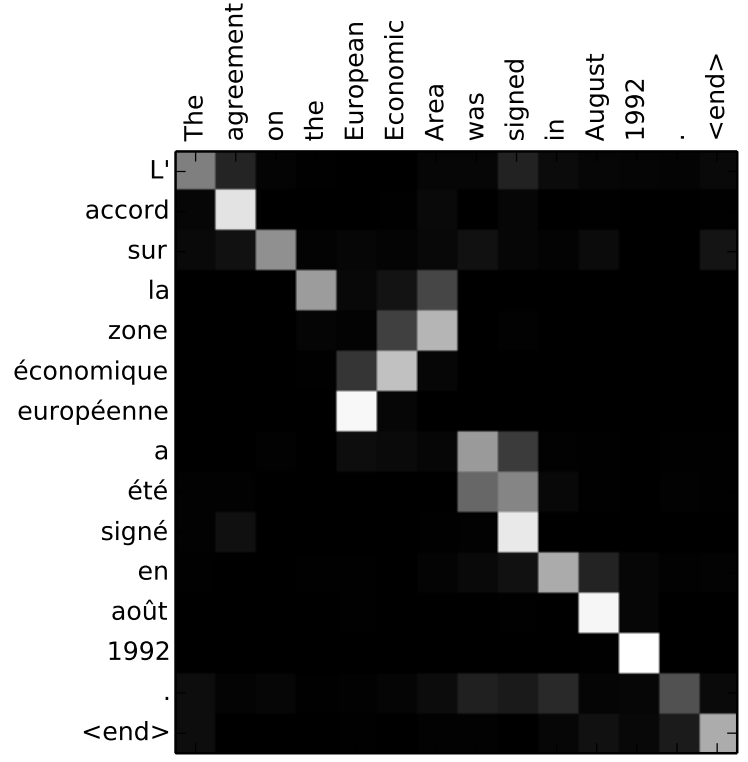
\includegraphics[width=0.35\linewidth]{./figures/bahdanau_att.png}
\end{figure}
{\scriptsize Figure taken from \citem{bahdanau2014neural} for illustration.\\
We will see the English to French translation model in the next section.}
\end{itemize}
\end{frame}

\begin{frame}{Attention computation}
\vspace{-3mm}
There are various ways to compute the similarity scores $\simi(q, k) \in \mathbb{R}$
between two vectors $q, k \in \mathbb{R}^{d \times 1}$:
\begin{itemize}
\item dot attention \citem{luong-etal-2015-effective}
\[
\simi(q, k) = q \bullet k = q^{\intercal} k
\]
\pause
\item scaled dot attention \citem{trafo}
\[
\simi(q, k) = \dfrac{q^{\intercal} k}{\sqrt{d}}
\]
\pause
{\small ($\sqrt{d}$ because if elements in $q$ and $k$ are i.i.d random variables with mean 0 and variance 1, $q^{\intercal} k$ has mean 0 and variance $d$.)}
\pause
\item MLP attention \citem{bahdanau2014neural}
\[
\simi(q, k) = w^{\intercal} \tanh(W [q, k] + b)
\]
where $W \in \mathbb{R}^{d \times 2d}$ and $w, b \in \mathbb{R}^{d \times 1}$ are trainable parameters.
\end{itemize}
%\begin{itemize}
%\item scaled dot attention works well while being \textbf{efficient} (simple dot product!).
%\item \emphbf{Multi-head attention} is often used.
%\begin{itemize}
%\item[-] Carry out multiple attention operations using separate parameters, and concatenate the results from each head.
%\item[-] \code{torch.nn.MultiheadAttention}
%\end{itemize}
%\end{itemize}
\end{frame}

\begin{frame}{Attention computation (cont'd)}
In practice:
\begin{itemize}
\item \textbf{Scaled dot attention} works well while being efficient, and it has no parameter.
\item \emphbf{Multi-head attention} is often used:
\begin{itemize}
\item[-] Split each of key/value/query vectors into $H$ sub-vectors. $H$ is the number of heads.
\item[-] Compute separate attention operations for each key/value/query sub-vectors.
\item[-] Concatenate (feature dimension) the results from each head to get the final output.
\end{itemize}
e.g., if the dimension is 512 (for each of key, value and query), and we use 8 attention \textbf{heads}, each attention computation is carried out for 64 dimensional sub-vectors.
\item \code{torch.nn.MultiheadAttention}
\end{itemize}
%\begin{itemize}
%\item scaled dot attention works well while being \textbf{efficient} (simple dot product!).
%\item \emphbf{Multi-head attention} is often used.
%\begin{itemize}
%\item[-] Carry out multiple attention operations using separate parameters, and concatenate the results from each head.
%\item[-] \code{torch.nn.MultiheadAttention}
%\end{itemize}
%\end{itemize}
\end{frame}



\begin{frame}{Attention with neural networks, applications}
\begin{itemize}
\item Originally proposed for machine translation (next section).
\item Intuition: focus only on parts of the input sentence, while producing parts of target sentence...
\item Impact on many other applications: attention is everywhere now.
\item \emphbf{Differentiable implementation of dictionary/database retrieval}.
\item Fundamental idea of \emphbf{ignoring irrelevant information}.
\item Visualization and interpretability.
\end{itemize}
% We will see more concrete examples later, and in the \emphbf{final exercise/assignment}.
\end{frame}



\begin{frame}{Self-attention\\ (autoregressive version)}
Can we build a general purpose sequence processing layer based on attention?
\begin{itemize}
\item Alternative to RNNs to process sequences.
\pause
\item {\small Note: autoregressive means that we process a sequence $x_1^N$ from left to right (or right to left) step by step:
i.e. while predicting a token $x_n$, we make use of information from the past $x_1^{n-1}$.}
\pause
\item Basic idea: ``enlarge the database for each new input"\\
\begin{itemize}
\item[-] Each input transformed in 3 ways: key, value, and query vectors.
\item[-] Store key and value vectors from all predecessor inputs (``database")
\item[-] Compute the output via attention using the query vector.
\end{itemize}
\pause
\item Does this make sense?
\end{itemize}
%\pause
%\vspace{3mm}
%Result of incremental refinements:
%\begin{itemize}
%\item \cite{cheng16}: Proposed as augmentation for LSTM
%\item \cite{ParikhT0U16}: Generic formulation.
%\item \cite{trafo}: Used in multiple layers in Transformer.
%\end{itemize}
\end{frame}

\begin{frame}{Self-attention, illustration}
\begin{figure}
\hspace{-10mm}
                        \centering
                        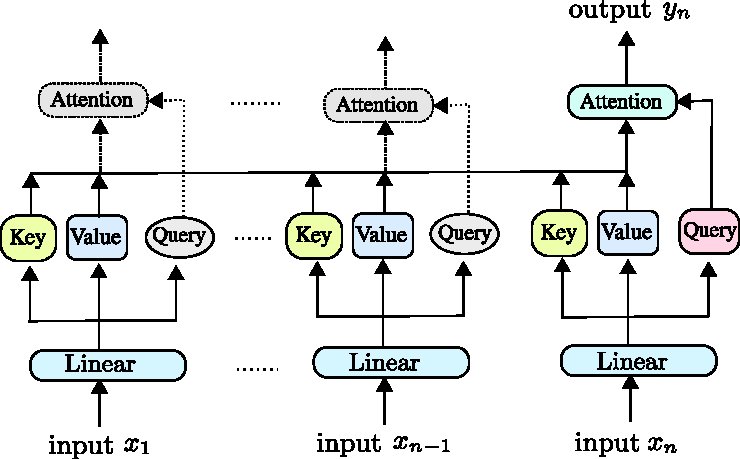
\includegraphics[width=.7\linewidth]{./figures/self_attention_only.pdf}
\end{figure}
\begin{itemize}
\item \textbf{Abandon compression} ability of RNNs!
\item Perform very well as a part of \emphbf{Transformer} models (up next).
\end{itemize}
\end{frame}

\begin{frame}{Self-attention (cont'd)}
\begin{itemize}
\item Consider a sequence of vectors ($x_1$, ..., $x_N$):
\pause
\item At step $n$, input $x_n \in \mathbb{R}^{D \times 1}$ is first projected into \emphbf{three} vectors:
   \begin{eqnarray*}
q_n, k_n, v_n = Qx_n, Kx_n, Vx_n \text{\hspace{8mm}} Q,K \in \mathbb{R}^{d_{\text{key}} \times D}, V \in \mathbb{R}^{d_{\text{value}} \times D}
    \end{eqnarray*}
$Q,K,V$ are the \emphbf{trainable parameters} of the layer.
\pause
\item The \emphbf{memory} of the layer consists of \emphbf{concatenation} of $k_i$ and $v_i$ vectors (along position/time dimension)
for all predecessor inputs. Thus, at step $n$:

\begin{eqnarray*}
\mathcal{K}_n &=& \Concat\!\big(\mathcal{K}_{n-1}, k_n) \in \mathbb{R}^{d \times n} \\
\mathcal{V}_n &=& \Concat\!\big(\mathcal{V}_{n-1}, v_n) \in \mathbb{R}^{d \times n} \\
\end{eqnarray*}
%which is:
%\begin{eqnarray*}
%h_n = \big(\mathcal{K}_n, \mathcal{V}_n\big) = \big((\mathcal{K}_{n-1}, k_n), (\mathcal{V}_{n-1}, v_n)\big)
%\end{eqnarray*}


%   \begin{eqnarray*}
%h_n = \big(\mathcal{K}_n, \mathcal{V}_n\big) = \big((\mathcal{K}_{n-1}, k_n), (\mathcal{V}_{n-1}, v_n)\big)
%    \end{eqnarray*}
\pause
State size $h_n = \big(\mathcal{K}_n, \mathcal{V}_n\big)$ increases with the sequence length; unlike in RNNs!
\pause
\item Output $y_n $ is computed by \emphbf{attention} using these vectors:
   \begin{eqnarray*}
y_n = \SelfAttention(h_{n-1},x_n) = \Attention(\mathcal{K}_n, \mathcal{V}_n, q_n)
    \end{eqnarray*}
\end{itemize}
\end{frame}

\begin{frame}{Self-attention, positional encoding}
\vspace{-4mm}
\begin{itemize}
\item One more concept needs to be introduced: \emphbf{positional encoding}.
\item Attention operation is invariant to shuffling key-value pairs \{($k_i$, $v_i$)\}$_{1 \leq i \leq N}$.
\item[-] Positional information needs to be provided explicitly.
\item[-] Positional encoding is a vector of the same size as input word/token embeddings,
representing the position.
\item We \textbf{add} the positional encoding vectors to the input embeddings.
\end{itemize}
\end{frame}

\begin{frame}{Self-attention, positional encoding (cont'd)}
\begin{itemize}
\item Common model: \emphbf{sinusoidal positional encoding}.\\ $e(i) \in \mathbb{R}^D$ representing the position $i \in \mathbb{N}$. Each component of $e(i)$ is computed as follows: for $0 \leq k < \dfrac{D}{2}$
                \begin{eqnarray*}
                        e(i)_{2k} = \sin(i/10000^{2k/D}) \\
                        e(i)_{2k+1} = \cos(i/10000^{2k/D})
                \end{eqnarray*}
\pause
Original motivation: $e(i+m)$ linearly depends on $e(i)$ \\(effective benefit of this property is not fully known).\\
The choice of ``10000": a \textit{large} number.
\pause
\item Standard approach: this vector is added (element-wise) to the input token/word embedding vector.
\pause
\item Studying and improving positional encoding has been also a common research topic
for self-attention based models.
\end{itemize}
\end{frame}

\begin{frame}[fragile]{Positional encoding, implementation}
\vspace{-5mm}
\begin{python}
class PositionalEncoding(nn.Module):
    """Example adapted from:

    https://pytorch.org/tutorials/beginner/transformer_tutorial.html
    """
    def __init__(self, d_model, max_len=5000):
        super(PositionalEncoding, self).__init__()
        self.max_len = max_len

        pe = torch.zeros(max_len, d_model)
        position = torch.arange(
            0, max_len, dtype=torch.float).unsqueeze(1)
        div_term = torch.exp(torch.arange(0, d_model, 2).float()
                             * (-math.log(10000.0) / d_model))
        pe[:, 0::2] = torch.sin(position * div_term)
        pe[:, 1::2] = torch.cos(position * div_term)

        # shape (max_len, 1, dim)
        pe = pe.unsqueeze(0).transpose(0, 1)
        self.register_buffer('pe', pe)  # Will not be trained.

# ... continue to next slide ...
\end{python}
\end{frame}


\begin{frame}[fragile]{Positional encoding, implementation (cont'd)}
\vspace{-5mm}
\begin{python}
# ... continue from previous slide ...

    def forward(self, x):
        # shape of x: (len, B, dim)
        assert x.size(0) < self.max_len, (
            f"Too long sequence: increase `max_len`")
        # shape of x (len, B, dim)
        x = x + self.pe[:x.size(0), :]
        return x

\end{python}
\end{frame}

\begin{frame}{Positional encoding, visualization}
\vspace{-5mm}
\begin{figure}
\centering
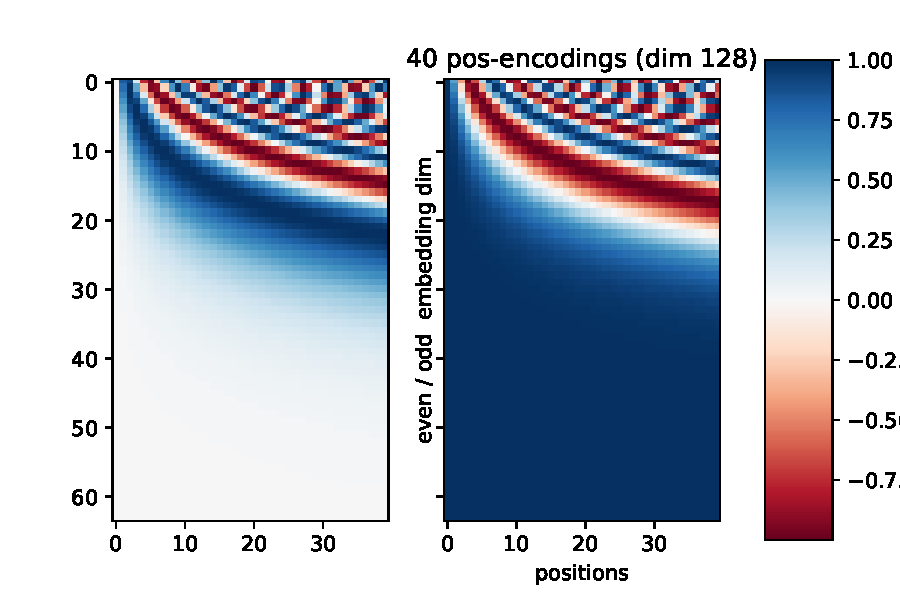
\includegraphics[width=.7\linewidth]{./figures/pos_enc.pdf}
\end{figure}
\begin{itemize}
\item Left: even, right: odd coordinates.
\item Positional information is encoded in a few coordinates:
\item[-] e.g., compare the vectors representing position \textit{0} vs. position \textit{30}.
\item This will be added to the token embedding vector.
\end{itemize}
\end{frame}


\begin{frame}{Transformer\\
(auto-regressive version)}
\vsp
\begin{minipage}{0.6\linewidth}
\begin{itemize}
\item One Transformer layer \citem{trafo} consists of multiple sub-layers:
\begin{itemize}
\item[-] One \emphbf{self-attention layer}
\item[-] One \emphbf{feed-forward layer}
\item[-] (We'll also add one \textit{cross attention layer} in the sequence-to-sequence version that we'll see next week!).
\end{itemize}
\vsp
\item with helper components which facilitate training:
\begin{itemize}
\item[-] \textbf{Residual connection} \\(which we have seen in the last section)
\item[-] \textbf{Layer normalization} \\(mean/variance normalization on feature dimension)
\end{itemize}
\end{itemize}
\vspace{3mm}

\end{minipage}
\begin{minipage}{0.35\linewidth}
\begin{figure}
\centering
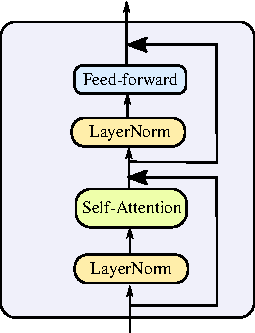
\includegraphics[width=.8\linewidth]{./figures/trafo_only.pdf}
\end{figure}
\end{minipage}
\vspace{5mm}
{\small Typical Transformer models has multiple layers (up to ~100; depending on the problem).}
\end{frame}

\begin{frame}{Transformer layer, illustration\\ (autoregressive case)}

Illustration with a Transformer language model\\ (as a generic example for sequence processing):

\begin{figure}
\hspace{-10mm}
                        \centering
                        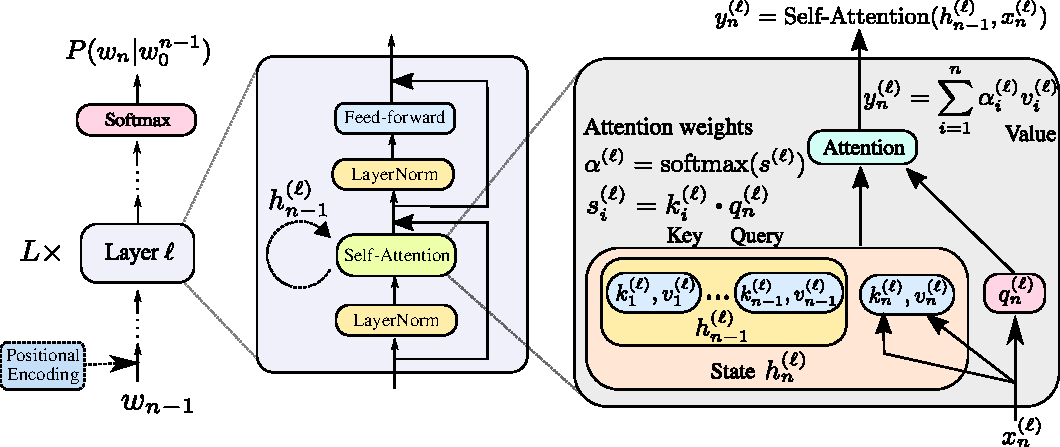
\includegraphics[width=.9\linewidth]{./figures/trafo_lm.pdf}
\end{figure}
Many impactful models, e.g. OpenAI's GPT-2 \& 3 models.
\end{frame}

\begin{frame}{Transformer (cont'd)}
\begin{itemize}
\item Made self-attention very popular.
\item Latest largest advancement in neural network architecture (2017).
\item You will be likely using a Transformer layer instead of self-attention layer alone.
\item \codeb{torch.nn.Transformer}: we will see this in details in the next chapter
\item The \textbf{final assignment} is about Transformers.
\end{itemize}
\end{frame}


% \begin{frame}[fragile]{Transformer, implementations}
% Relevant functions (from PyTorch $\geq$ 1.2, but many changes since then: use 1.6.0):
% \begin{itemize}
% \item \codeb{nn.Transformer}: transformer model.
% \item \codeb{nn.TransformerEncoder}: stack of N encoder layers
% \item \codeb{nn.TransformerDecoder}: stack of N decoder layers
% \item \codeb{nn.TransformerEncoderLayer}: made up of self-attention and feed-forward network.
% \item \codeb{nn.TransformerDecoderLayer}: made up of self-attention, multi-head-attention and feedforward network.
% \item \codeb{nn.MultiheadAttention}
% \item For positional encoding, see e.g. \link{https://pytorch.org/tutorials/beginner/transformer_tutorial.html}
% \end{itemize}
% We will see "encoder-decoder" concept in the next Chapter.
% \end{frame}


\begin{frame}{Summary}
\textbf{What have we learned?}
\begin{itemize}
\item Different neural network architectures for different problems.\\ Key words:
\begin{itemize}
\item Convolutional neural networks
\item Recurrent neural networks
\item Long short-term memory
\item Attention
\end{itemize}
\item Intuitions reflected in the design of these models.
\end{itemize}
\vsp
\textbf{Coming up next...}
\begin{itemize}
\item How to build complete model for different problems using these building blocks (next Chapter)
\end{itemize}
\end{frame}
